\documentclass[11pt,english,a4paper]{article}
\usepackage{natbib, amsmath, amsfonts, units, graphicx, hyperref, txfonts, fleqn, geometry, pifont, setspace, eurosym, afterpage, caption}
\usepackage{fancyhdr}

% Override daft defaults for float positioning
\renewcommand{\topfraction}{0.9}	% max fraction of floats at top
\renewcommand{\bottomfraction}{0.8}	% max fraction of floats at bottom
% -- Text pages
\setcounter{topnumber}{2}
\setcounter{bottomnumber}{2}
\renewcommand{\textfraction}{0.07}
% -- Float pages
\renewcommand{\floatpagefraction}{0.7}

\providecommand{\keywords}[1]{\textbf{\textit{Keywords ---}} #1}
\renewcommand*{\bibfont}{\small}
\setlength{\bibsep}{0.0pt}

\captionsetup[figure]{labelfont={small,bf},textfont=small,justification=raggedright,labelsep=space,singlelinecheck=false}
\captionsetup[table]{labelfont={small,bf},textfont=small,justification=raggedright,labelsep=space,singlelinecheck=false}

\pagestyle{fancy}
\fancyhf{}
\lhead{Smith LS \textit{et al.} (2014)}
\rhead{}
\cfoot{\thepage}

\title{Towards a hydrodynamic modelling framework appropriate for applications in urban flood assessment and mitigation using heterogeneous computing}
\author{Luke S. Smith,\\
	Civil Engineering and Geosciences,\\
	Newcastle University\\
	\texttt{l.s.smith@ncl.ac.uk}
	\thanks{Telephone: +44 (0) 191 208 6766}
\and
	Qiuhua Liang,\\
	Civil Engineering and Geosciences,\\
	Newcastle University\\
	\texttt{qiuhua.liang@ncl.ac.uk}
\and
	Paul F. Quinn,\\
	Civil Engineering and Geosciences,\\
	Newcastle University\\
	\texttt{p.f.quinn@ncl.ac.uk}
}
\date{\vspace*{12.0pt}Accepted \textbf{19 June 2014} \\ Published online \textbf{31 July 2014}}

\begin{document}
\maketitle

\begin{abstract}
We present a new hydrodynamic modelling framework capable of fully exploiting modern graphics and central processing units (GPUs and CPUs) from any of the mainstream vendors, to be used in the design and assessment of sustainable drainage systems. A finite-volume Godunov-type scheme is combined with the HLLC Riemann solver to create a robust numerical model which correctly addresses wetting and drying and transient flow conditions, and is suitable for application to a wide range of flood simulations. The software is tested with a three day flood event in Carlisle during 2005, at resolutions from 25m to 2m. Run-times are significantly reduced without compromising numerical accuracy. Excellent agreement is found between the simulation results and a comprehensive post-event survey. Changes in sensitivity to Manning's \(n\) are examined at different resolutions, with changes to the floodplain found to have little influence at 2m resolution.
\end{abstract}
\keywords{graphics processing unit (GPU), finite-volume Godunov-type scheme, shallow water equations, urban flooding, sustainable urban drainage}

\vfill
\noindent\fbox{
\begin{minipage}{\dimexpr\textwidth-2\fboxsep-2\fboxrule}
\small
This is the authors' version of a work that was accepted for publication in Urban Water Journal. A definitive version was subsequently published in Urban Water Journal online. doi:\url{http://dx.doi.org/10.1080/1573062X.2014.938763}
\end{minipage}
}

\section{Introduction}

The United Kingdom was subjected to numerous storms and severe floods throughout 2012, the wettest year for a century, resulting in lives lost and millions of pounds worth of damage. The UK was not alone, with similarly unusual weather events reported across the globe. As an example, in June 2013 an extreme flood event affected a substantial area of central Europe, resulting in 25 deaths and more than \euro{12bn} losses. This is not a new problem; the UK Environment Agency attributed two thirds of flooding during 2007 when a similarly wet season caused widespread disruption, to surface water and inadequacies in drainage \citep{Pitt2007}. In England alone over 5.2 million properties are known to be at risk of flooding, and annual investment must increase to more than a billion pounds per year just to maintain current levels of protection under the threat of climate change \citep{EnvironmentAgency2009a}. 

Attenuation of rainwater to reduce hydrograph peaks and alleviate surface water flooding is best achieved by sustainable drainage systems (SuDS) in urban areas. Comprehensive guidance is provided in the UK for the design and management of these by \citet{Woods-Ballard2007}. This stipulates that designs should consider and protect against overland flow originating off-site, and that the consequences of drainage blockage should be simulated. Such simulations are difficult to accomplish in practice, requiring high-resolution modelling of runoff source areas and all potential pathways to the site. Assessing the likely impacts of the proposed SuDS requires similarly high resolutions to represent the complex flow dynamics which might occur in wet ponds and infiltration basins, and to consider rates of sedimentation and maintenance requirements. Further complications are introduced by simulating hypothetical events affecting developments which have not and hopefully never will flood, meaning there is scarce data against which a parametric calibration might be performed. Where SuDS are in place, the residual risk remaining if the design storm is exceeded must be quantified to meet the recommendations of \citet{Pitt2007}.

Whilst the required high-resolution topographic data is increasingly available from airborne altimetric LiDAR, its wider application across large urban extents has largely been constrained by limitations in computational power and the performance of hydraulic modelling software. Research has understandably focussed in recent years on establishing how software models might be accelerated. Different techniques have been applied, such as dynamically adaptive grids, spatially-varying timesteps, and simplified approximations for the physics, with a particular emphasis on the latter. Dynamically adaptive grids retain the physical complexity but introduce new challenges in strictly maintaining both mass and momentum conservation, and will rarely increase the timestep if the most complex flow dynamics are represented at the highest resolutions \citep[e.g.][]{Liang2008,Kubatko2009}. A spatially-varying timestep complicates evaluation of inter-cell fluxes where cells have differing simulation times (Sanders 2008, Trahan and Dawson 2012); furthermore, the efficiency gain does not always balance the workload associated with implementing a considerably more complex software structure. 

Elimination of terms from the shallow water equations (SWEs) gives rise to kinematic and diffusive wave approximations. These may allow faster computation at the expense of losing physical complexity, but compromise the predictive capabilities for flow velocity and by extension the time of inundation. Diffusive approximations are hindered at high resolutions by a strict timestep constraint, and kinematic approximations neglect potentially significant aspects of flow such as backwater effects \citep{Bates2000,Tsai2003,Hunter2005}. The topographic features of urban environments are characterised by narrow gaps between buildings and steep gradients; such conditions all have the potential to create transient flows, increase velocities, induce shocks, and cause backwater effects \citep{Testa2007,ElKadiAbderrezzak2011,Xia2011}. Comprehensive analysis of simplified approaches and the errors therein from numerical and pragmatic perspectives is given by \citet{Singh1996a}, \citet{Hunter2007}, and \citet{Pender2010,Pender2013}. Simplified models are known to produce good results when calibrated against observed inundation data \citep[e.g.][]{Neal2009,Horritt2010} but parametric uncertainty and sensitivity is problematic for simulating hypothetical events \citep{Horritt2002,Yu2006,Fewtrell2008a}, as required for SuDS design.

Whilst transistor counts on central processing units (CPUs) continue to rise at rates comparable to Gordon Moore's observations, clock speed increases have stalled. Software developers must increasingly look to multi-core processing if they are to fully leverage the power of modern computers. Despite this a large number of commercial hydraulic modelling packages provide no such functionality, even though good weak and strong scaling can be accomplished \citep{Sanders2010,Kalyanapu2011,Sætra2012a}. Heterogeneous computing and the advent of new methods (i.e. CUDA, OpenCL, DirectCompute) of interfacing with graphics processing units (GPUs) are even more promising: these devices are well-suited to performing the same calculation across large datasets, and are ideal for computational fluid dynamics (CFD). Much of the literature focuses on CUDA implementations which are constrained to operating on NVIDIA hardware \citep[e.g.][]{Kuo2011,Sætra2012a}. Commercial software options for hydraulic modelling on GPU architectures are now available; a comparison can be found in \citet{Pender2013}, albeit limited to small domains which cannot fully capitalise on the parallel processing benefits \citep{Sætra2012a}. The majority have yet to be released to the public, and all those the authors are aware of utilise CUDA and are hence limited to operating on NVIDIA hardware. Herein we describe how OpenCL allows a single codebase to be used for parallel computation with either CPU or GPU devices available any of the mainstream vendors. 

The work of \citet{Ozdemir2013} explicitly considers the benefits of high-resolution modelling for SuDS design, emphasising that increased topographic detail improves results beyond the range of parametric calibration. Simulation run-times and instabilities are recognised therein as barriers to wider application, but nonetheless best practice guidance encourages the use of detailed hydraulic modelling for long-term storage design \citep{Woods-Ballard2007}. Herein, we contribute towards resolving both of these problems. We describe how a robust finite-volume Godunov-type scheme is implemented for new software, and applied to simulate flow dynamics during a flood at the whole-city scale with a high-resolution grid. 

\section{Methodology}

We first consider a numerical scheme appropriate for use in urban flood modelling. As a minimum the scheme must appropriately address complex flow dynamics for transient flow conditions where shocks may be present. It must also be able to handle cell wetting and drying, depict a lake at rest even with uneven bed topography, and preserve depth positivity. We then transpose the approach to a computational framework suitable for parallel execution with various types of processing device. 

\subsection{Finite-volume Godunov-type scheme}

It is generally true that the vertical scale of the fluid flows is much smaller than the horizontal for flood events. It is therefore appropriate to approximate the flood wave dynamics with the SWEs derived by depth integrating the Reynolds-averaged Navier-Stokes equation. This hyperbolic system of conservation laws accounts for both mass and momentum conservation, and is presented in vector notation as

\begin{equation}
	\label{SWE}
	\frac{\partial\textbf{U}}{\partial t} +
	\frac{\partial\textbf{F}}{\partial x} +
	\frac{\partial\textbf{G}}{\partial y} =
	\textbf{S} ,
\end{equation}

where t is the simulation time, \(x\) and \(y\) refer to the Cartesian coordinate space, \(\textbf{U}\) is the vector of flow variables, \(\textbf{F}\) and \(\textbf{G}\) are fluxes in the two respective Cartesian dimensions, and \(\textbf{S}\) is a source term vector through which inflow and losses may be accounted for. The equation is solved within a regular two-dimensional Cartesian domain, for which the vector terms of equation \eqref{SWETerms} are as described in \citet{Liang2009b}, 
 
\begin{equation}
	\label{SWETerms}
	\begin{alignedat}{4}
		&\textbf U && = \left[ \begin{array}{c}
			\eta \\
			uh \\
			vh
		\end{array} \right] , ~ &&
		\textbf F &&  = \left[ \begin{array}{c}
			hu \\
			hu^2 + \frac{1}{2}(g\eta^2 - 2\eta z_b) \\
			huv
		\end{array} \right] ,\\
		&\textbf G && = \left[ \begin{array}{c}
			hv \\
			hvu \\
			hv^2 + \frac{1}{2}(g\eta^2 - 2\eta z_b) \\
		\end{array} \right] , ~ &&
		\textbf S && = \left[ \begin{array}{c}
			0 \\
			-\frac{\tau_bx}{\rho} - g\eta \frac{\partial z_b}{\partial x} \\
			-\frac{\tau_by}{\rho} - g\eta \frac{\partial z_b}{\partial y} \\
		\end{array} \right] .
	\end{alignedat}
\end{equation}

Here, \(\eta\) and \(z_{b}\) are the free surface level and bed elevation for the underlying topography respectively; \(h = \eta - z_{b}\) gives the total water depth; for the two Cartesian directions, \(u\) and \(v\) are depth-averaged velocities, \(qx (=uh)\) and \(qy (=vh)\) are volumetric discharge per unit width, \(\tau_{bx}\) and \(\tau_{by}\) are bed shear stresses, \(\partial{z_{b}} / \partial{x}\) and \(\partial{z_{b}} / \partial{y}\) define the bed slopes; \(g\) is acceleration due to gravity, \(\rho\) is the water density; and \(q_{0}\) denotes a source or sink for mass (e.g. rainfall, drainage outfall, etc.).

A Godunov-type scheme is used to solve equation \eqref{SWE} and ensure complex flow dynamics are represented (e.g. hydraulic jump transitions). Local solutions to the Riemann problem across each cell interface are hence used to update each cell state with the time-marching formula,

\begin{equation}
	\label{GodunovUpdate}
	\begin{alignedat}{2}
	\textbf{U}^{t+\Delta t} = \textbf{U}^t & - \frac{\Delta t}{\Delta x}(\textbf{F}^+ - \textbf{F}^-) 
					     &  - \frac{\Delta t}{\Delta y}(\textbf{G}^+ - \textbf{G}^-) + \Delta t \textbf{S} , 
	\end{alignedat}
\end{equation}

where \(\textbf{F}^-\), \(\textbf{F}^+\), \(\textbf{G}^-\), \(\textbf{G}^+\) are fluxes through a cell's western, eastern, southern and northern interfaces respectively. As a result of the explicit numerical scheme, the timestep \(\Delta{t}\) is constrained as per the conditions described by \citet{Courant1967},

\begin{equation}
	\label{CFL}
	\Delta t \le C \cdot min \left[\frac{\Delta x}{\lvert u + \sqrt{gh} \rvert} , \frac{\Delta y}{\lvert v + \sqrt{gh} \rvert}\right] ,
\end{equation}

where \(0 < C \le 1\). Depth positivity is preserved through reconstruction of the interface state pair before computing fluxes \citep{Liang2010b}, for which a piecewise distribution of flow information is assumed, allowing a single bed elevation and current conditions to be identified as

\begin{equation}
	\label{Reconstruction1}
		\hat{h}^L = \hat{\eta}^{L} - \hat{z_{b}}^{L}, \hfill
		\hat{u}^L = \hat{q_x}^{L} / \hat{h}^{L}, \hfill
		\hat{v}^L = \hat{q_y}^{L} / \hat{h}^{L}, \hfill and \hfill
		z_b = max( \hat{z_b}^{L} , \hat{z_{b}}^{R} ) , \hfill
\end{equation}

where superscript \(L\) and \(R\) indicate sides of the interface, and \(\hat{}\) indicates the values before reconstruction. From here the new discharge per unit width and free-surface levels are deduced,

\begin{equation}
	\label{Reconstruction2}
		h^L = max( 0, \hat{\eta}^{L} - z_{b} ), \hfill
		\eta^L = h^L + z_b, \hfill
		q_x^L = \hat{u}^L\hat{h}^L, \hfill and \hfill
		q_y^L = \hat{v}^L\hat{h}^L . \hfill
\end{equation}

Finally, a local bed modification is applied to ensure the free-surface level does not fall below the bed elevation, a condition which would otherwise give rise to spurious fluxes,

\begin{equation}
	\label{Reconstruction3}
		\Delta{z} = max( 0, z_{b} - \hat{\eta}^{L} ), \hfill
		z_b \gets z_b - \Delta{z}, \hfill and \hfill
		\eta^L \gets \eta^L - \Delta{z} . \hfill
\end{equation}

The process is similarly repeated for the right side of the cell interface. These reconstructed state values for both sides of a cell interface define local Riemann problems, solved by the HLLC approximate solver to obtain fluxes, thereby accounting for physical features of discontinuities including contact and shear waves \citep{Toro1994} and shown to perform well with differing flow conditions \citep{Erduran2002a}. The bed slope component of the source term vector in \eqref{SWETerms} is approximated through a central differencing approach. 

The friction source terms are solved independently of the main scheme using a point-implicit approach obtained through Taylor expansion, as proposed by \citet{Liang2010b}. 

\subsection{Software framework for CPU and GPU computation}

\begin{figure*}[tpb]
\centering
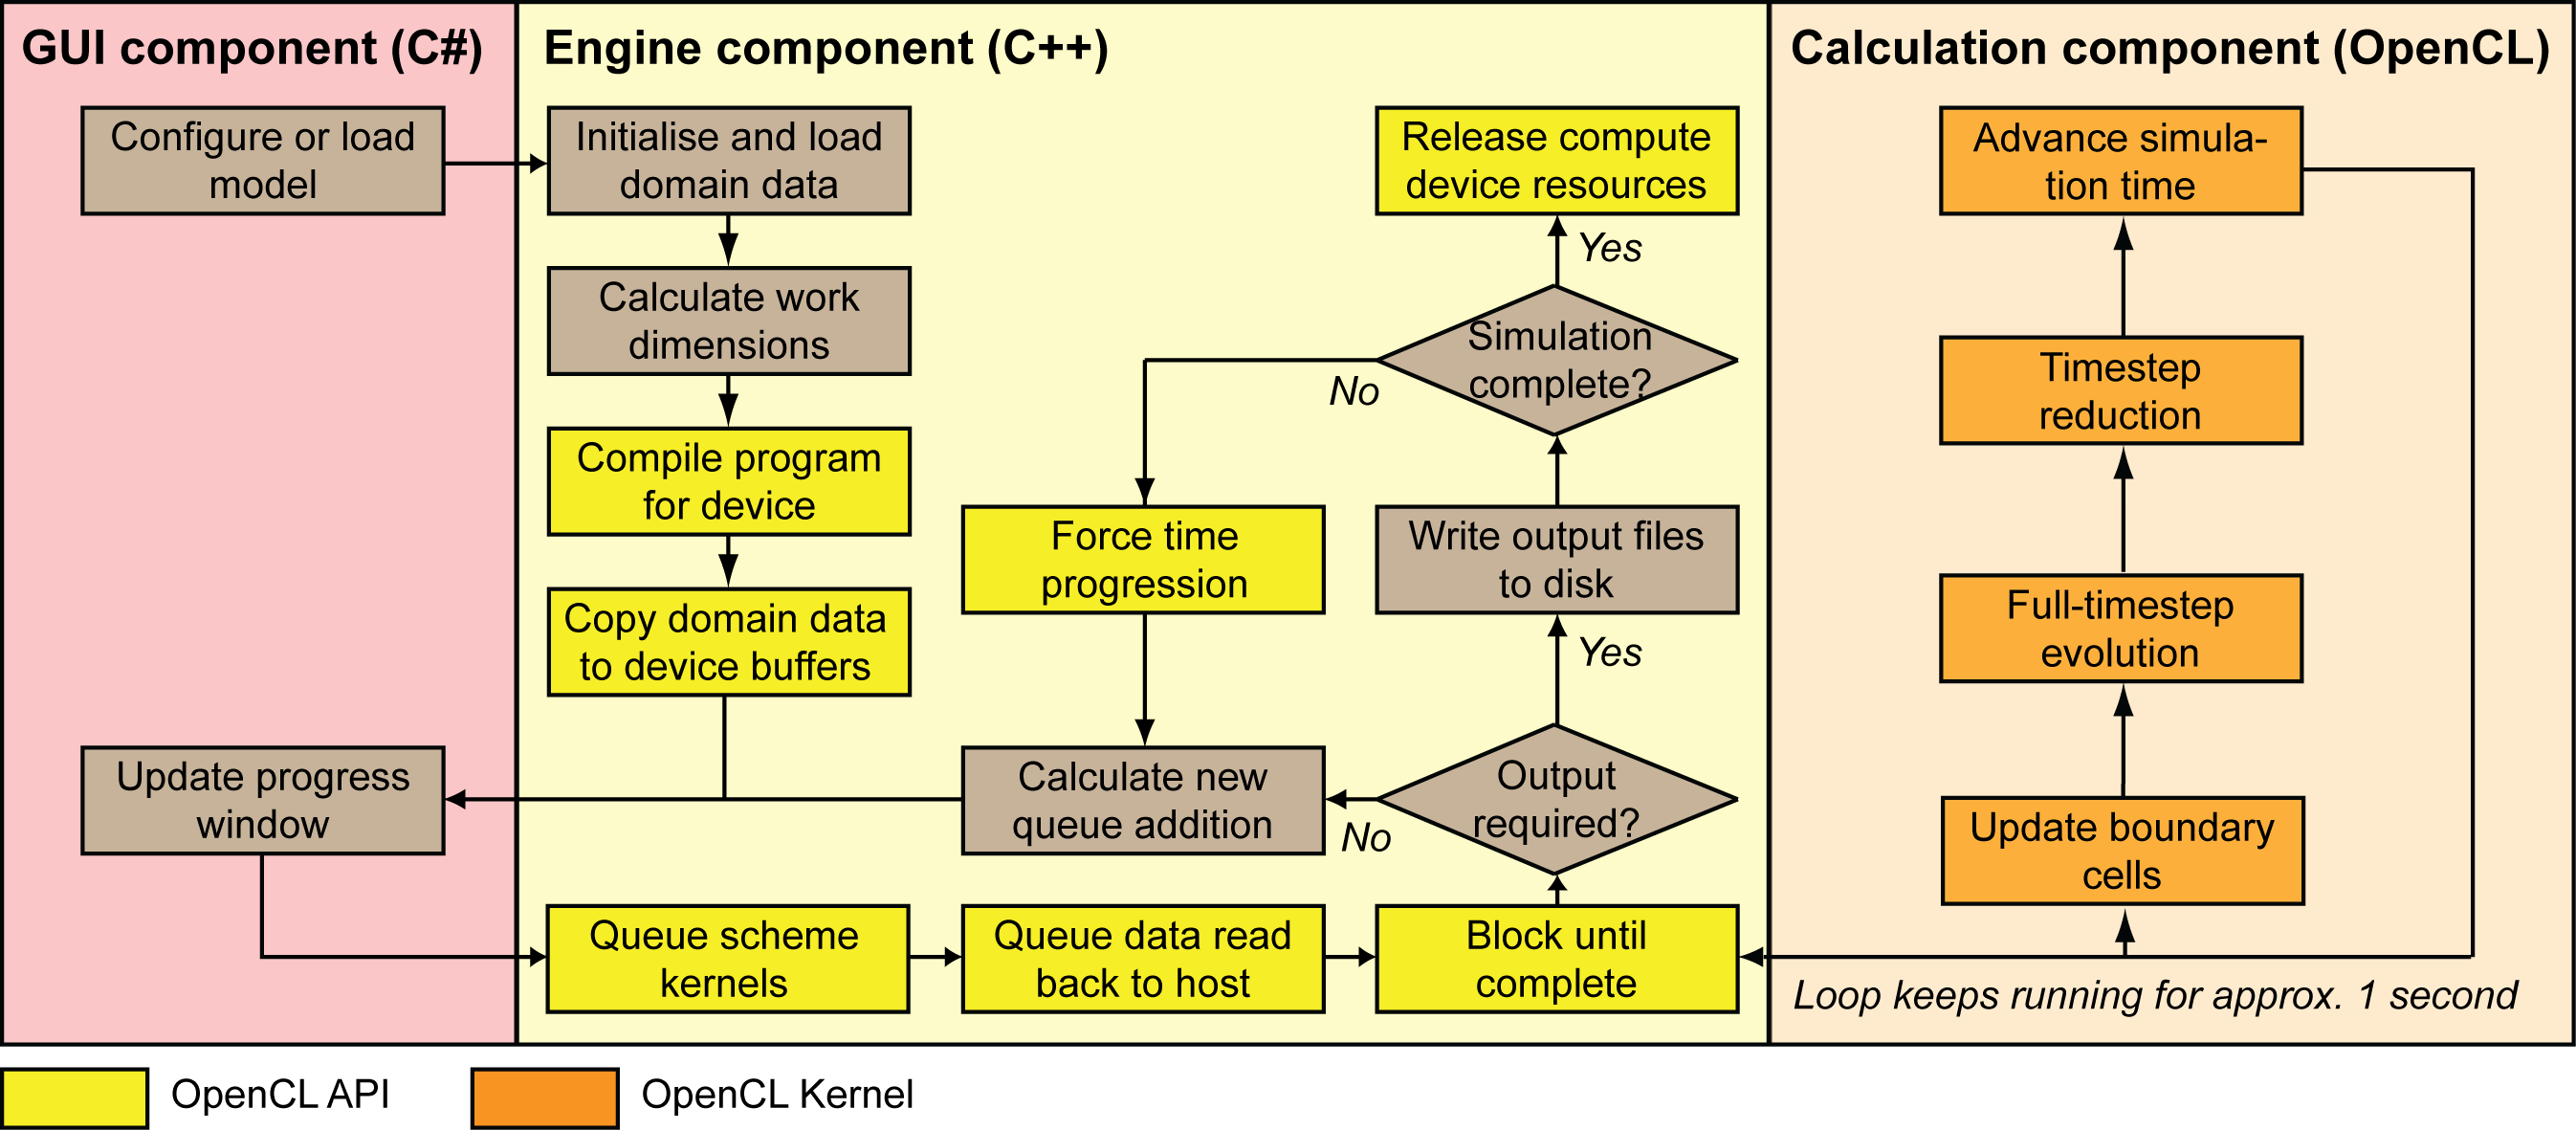
\includegraphics[width=1.0\textwidth]{Figure1.png}
\caption{Graphical representation of the software structure and main processes.}
\label{SoftwareProcesses}
\end{figure*}

Achieving high levels of performance for GPU devices requires careful consideration of the program structure and resource consumption in order to fully harness different processor architectures. Optimal levels of performance are achieved if a processing device is consistently occupied with work, allowing data transfers from global device memory (RAM) to processing unit specific registers to occur asynchronously in the background and the significant latency associated therewith to be masked. The underlying hardware manages the synchronisation of work across the resources available through the similar concepts of warps (NVIDIA) and wavefronts (AMD). Processing devices may only access data held within their own respective memories, thus duplicate copies of the domain data are required to reside in both GPU and CPU memory. Transferring data over the main system bus is an expensive operation, which should be as infrequent as possible.

The domain is considered as a single Cartesian grid with data stored in linear memory structures. 64-bit floating-point computation requires 48 bytes per cell including friction coefficients, which allowing for further constraints imposed by the device, permits up to 50 million cells per domain with GPU devices currently available before the maximum OpenCL buffer size is likely to be exceeded. Computation of larger domains within a single device would remain possible if cell data was split across multiple memory buffers. The numerical scheme is mapped to a series of small discrete programs (i.e. kernels in OpenCL terminology) which may run sequentially for multiple iterations before any data needs to be transferred back to the CPU. This allows efficient execution, with data transferred approximately every second to update the user on simulation progress, and write output files to disk if required. As a whole the software is structured as three discrete application elements of differing programming languages; a graphical representation of this model is shown in Figure \ref{SoftwareProcesses}: the graphical user interface is responsible only for allowing the user to configure a model, and providing status updates; the engine component is responsible for loading the required data, identifying suitable devices to be used in computation, coordinating the work required for the simulation, and writing output files at a user-defined interval. The calculation component is wholly parallelised, but to alleviate potential inefficiency resulting from the latency associated with host-bus transfers to GPU devices, several iterations of the numerical scheme can be scheduled to run independently before the engine component becomes aware of progress. This loop in the calculation component typically runs for approximately one second after the blocking command is issued in the engine component, after which it is assumed the user should be updated on simulation progress; the number of iterations is therefore a function of the size of the domain.

The scheme is effectively programmed as a stencil operation, for which the kernel is executed across every cell in the domain, but each requires data from its four immediate neighbours. Two memory buffers hold transient cell data as four-element vectors (consisting free-surface level, maximum level, and unit-width discharge in the x- and y-directions). The buffers are swapped each time the scheme kernels are queued (i.e. the target memory becomes the source memory for the next iteration). The outer-most layer of cells is exempt from the full-timestep evolution kernel, allowing these cells to provide reflective or transmissive boundary conditions. Only a first-order solution is used herein; a GPU implementation of the second-order accurate MUSCL-Hancock scheme within the same framework, and more in-depth discussion of the challenges for achieving computational efficiency can be found in \citet{Smith2013}. Boundary conditions are imposed directly at ghost cells exempt from processing at the edge of the computational domain, as in \citet{Liang2010b}.

\begin{figure*}[tpb]
\centering
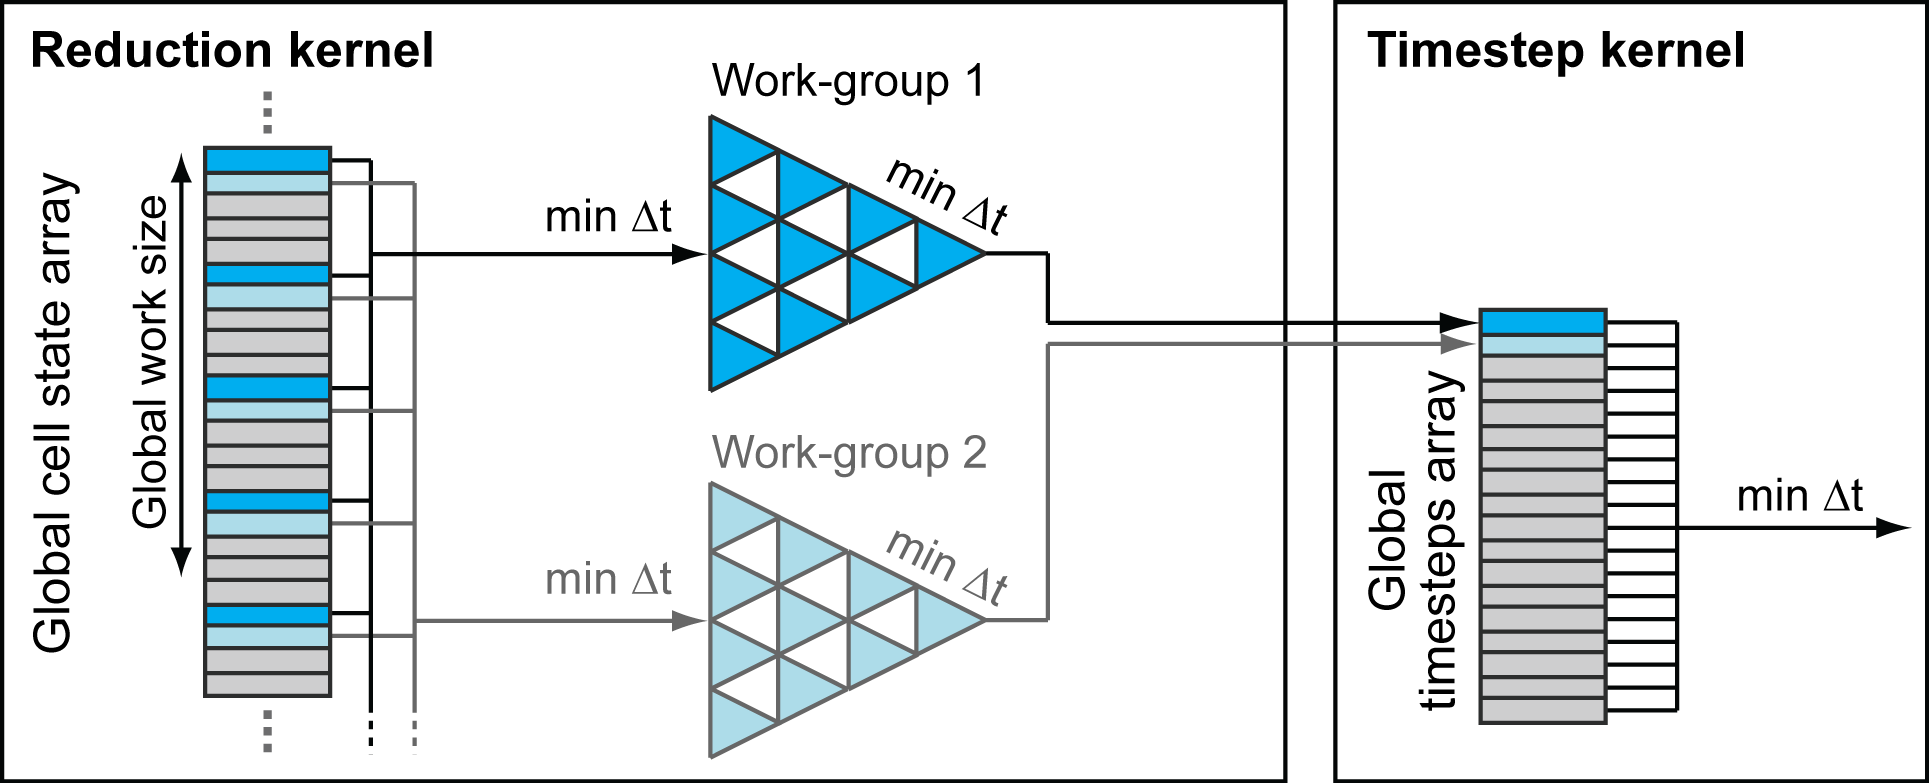
\includegraphics[width=0.8\textwidth]{Figure2.png}
\caption{Illustration of the reduction two-stage reduction process used to identify the timestep.}
\label{ReductionDiagram}
\end{figure*}

Implementation of the timestep constraint given in equation (4) requires identification of the greatest velocity present in the domain after each iteration of the numerical scheme, to create a variable timestep thus ensuring the stability of the numerical scheme. A two-stage reduction (i.e. identifying the minimum permissible timestep from a large number of cells) process adopted herein allows a large enough quantity of work per compute unit to mask memory latency through smaller but more intensive work dimensions. Domain cells are sampled with a regular stride until the end of the cell array is reached, then successive binary comparisons are carried out in multiple iterations until other threads within the group have been retired and a single value remains. This is carried forward to a new much smaller array of potential timesteps, which is examined finally when the simulation time is advanced. The process is illustrated in Figure \ref{ReductionDiagram}. The timestep is constrained to 0.1 seconds for the first minute of the simulation while the first water enters the domain. 

A perhaps unusual approach is adopted with OpenCL, allowing the code for the numerical scheme to be dynamically generated and complied at the point of use by the underlying system drivers with an instruction set specific to the hardware available. This allows code which is not required or disabled (e.g. second-order accuracy, friction effects) to be omitted altogether, and constants such as the domain dimensions to be stored within the program binary. The compiler is instructed to adhere to all of the appropriate IEEE standards for floating-point computation, hence standards-compliant CPUs and GPUs alike should produce identical results.

\section{Results and discussion}

The new software has been applied to simulate flooding in Carlisle, North West England, in January 2005. Over 200mm of rain fell in a few hours over the Cumbrian mountains, believed to be equivalent to a \(1\%\) annual exceedance probability (AEP) event. Rivers quickly responded, with a volumetric discharge exceeding 1,500 m\textsuperscript{3}s\textsuperscript{-1} recorded within Carlisle itself on the River Eden. Severe flooding ensued, in an event that played out over more than 48 hours, affecting over 6,000 residents and directly flooding over 1,900 properties \citep{GONW2005,EnvironmentAgency2006a}. This event is selected to test the model because of its excellent validation dataset and complex urban topography, however the authors stress that the software framework can similarly be used with pluvial boundary conditions for surface water flooding. 

In the week that followed both the Environment Agency (EA) and Bristol University conducted differential global positioning system (DGPS) surveys of water and wrack marks, their combined efforts creating one of the most comprehensive validation datasets for modelling urban flood inundation with 263 individual points. Different software codes and modelling techniques have since been applied to reproduce the event, most notably \citet{Neal2009}, \citet{Horritt2010}, \citet{Fewtrell2011a} and \citet{Liu2013}. 

\begin{figure*}[tpb]
\centering
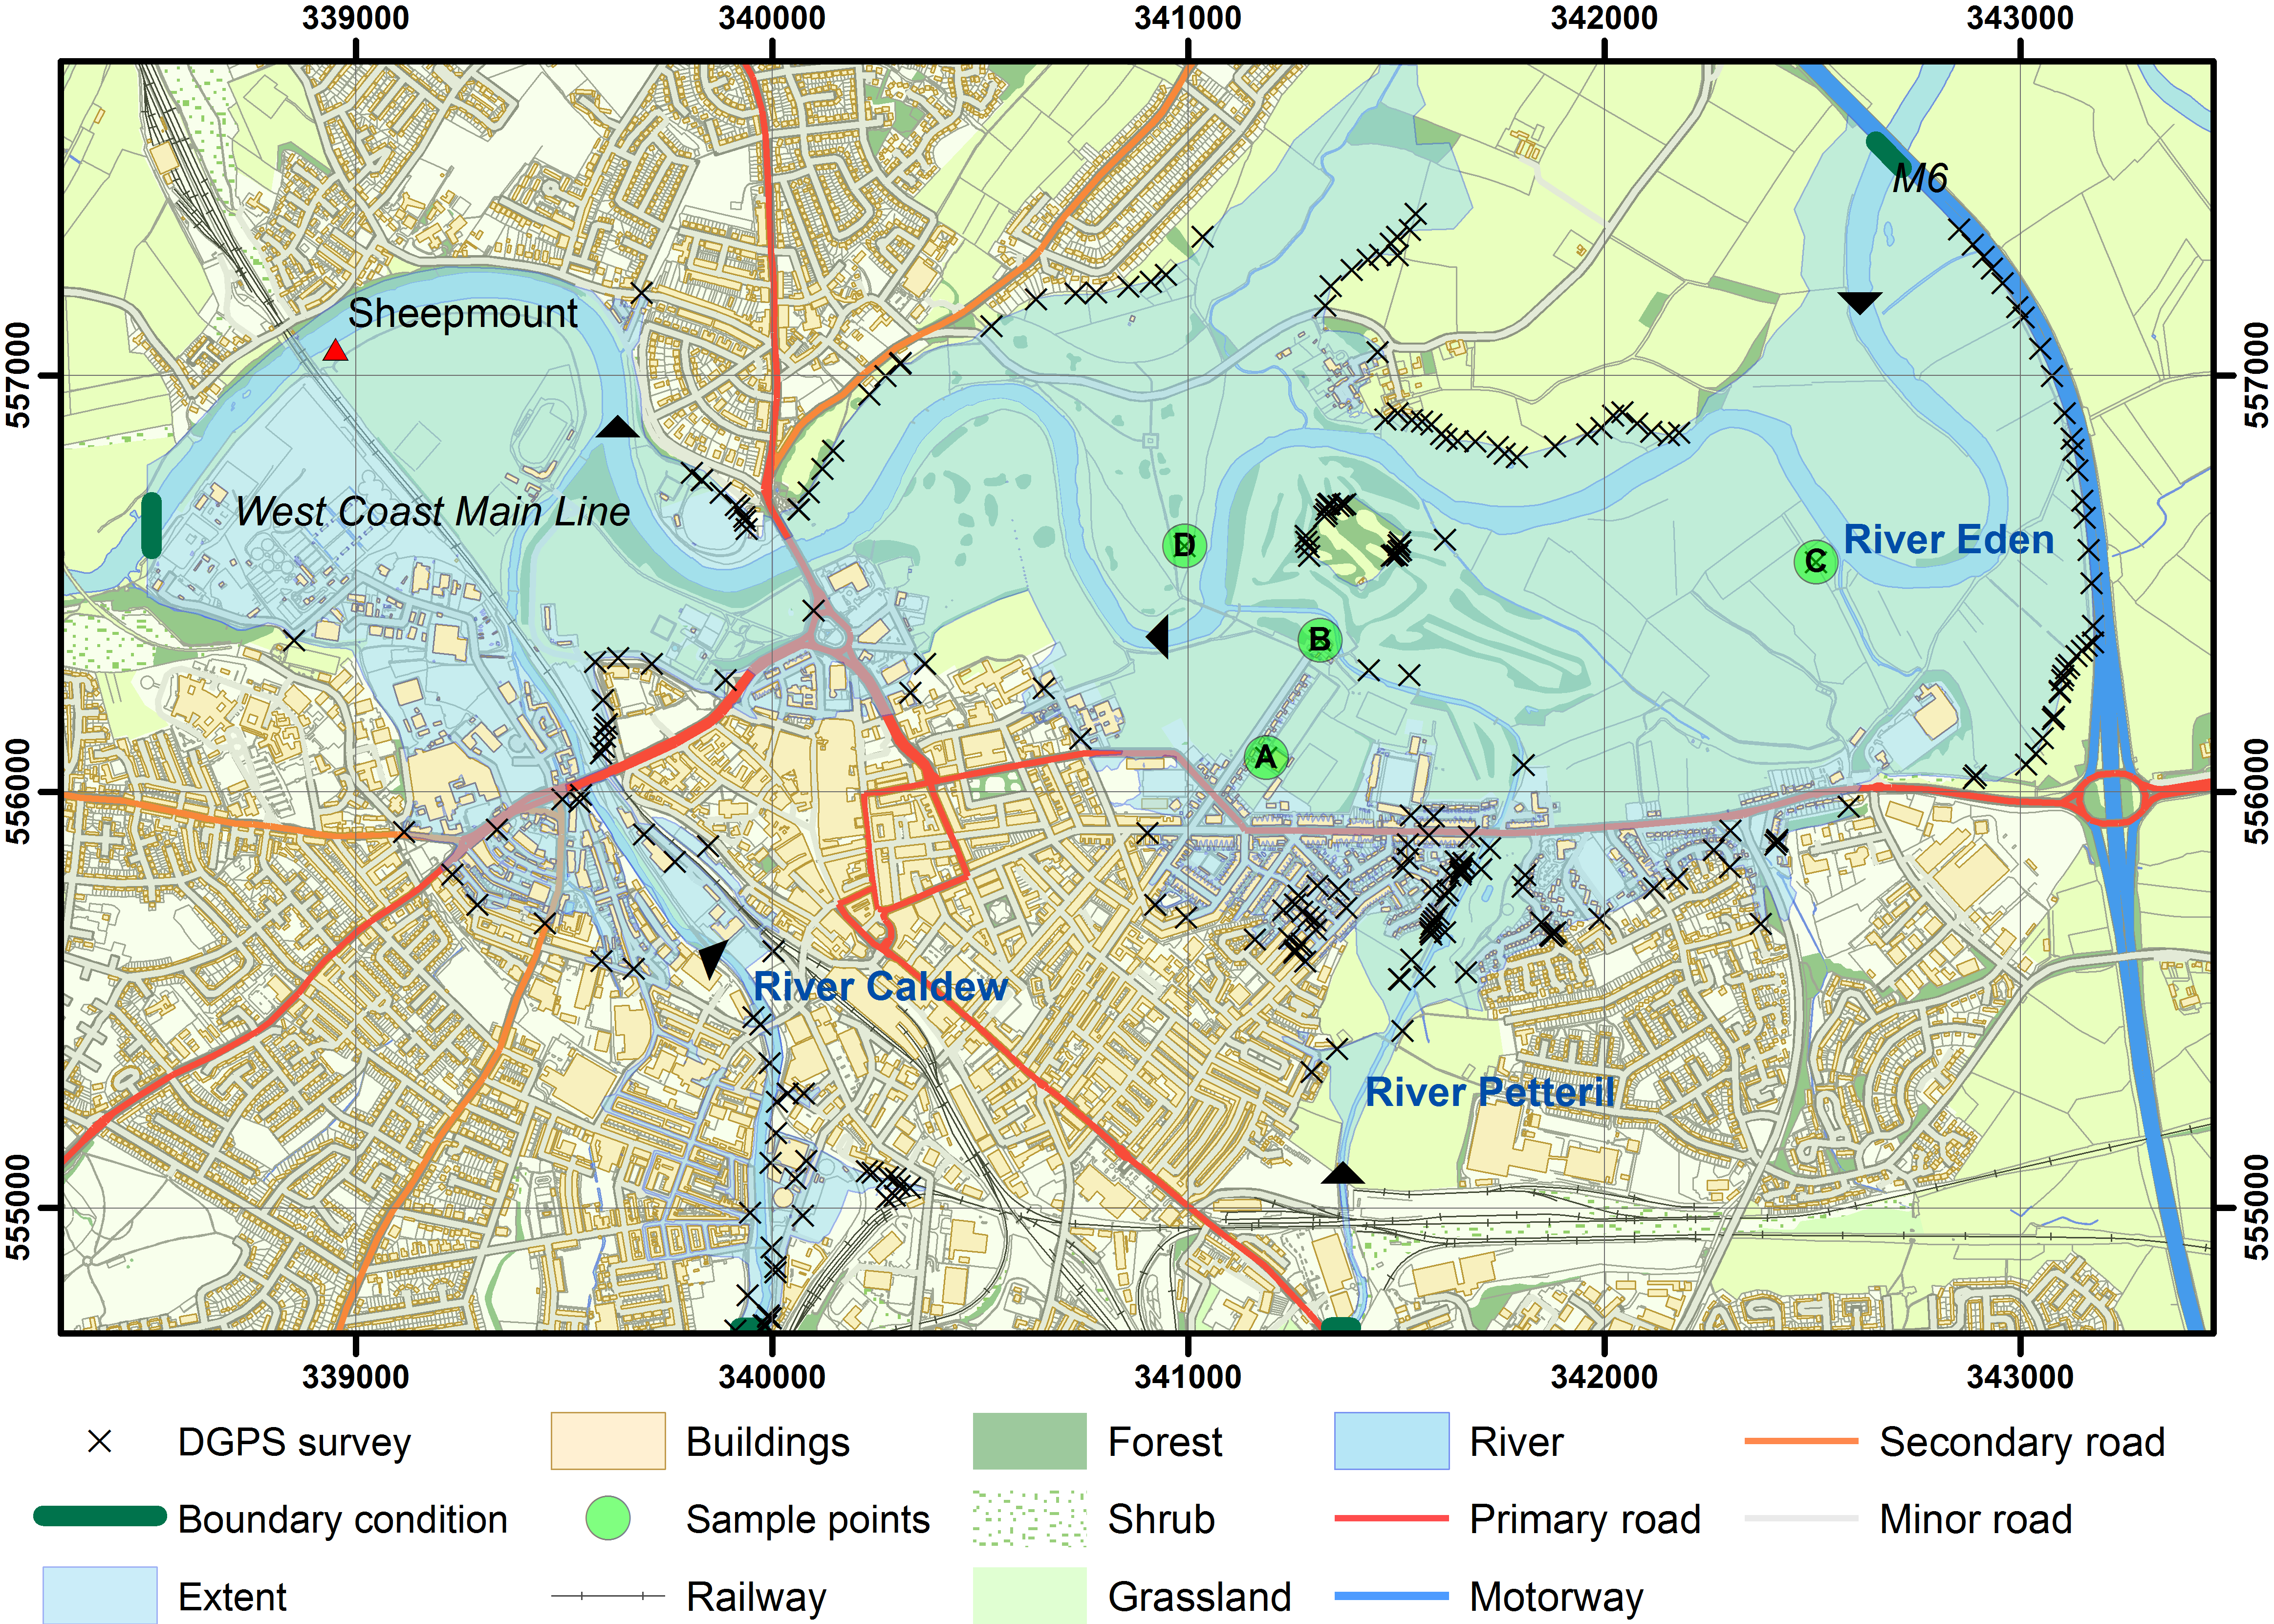
\includegraphics[width=1.0\textwidth]{Figure3.png}
\caption{Extent and topographic features for Carlisle with the three rivers and flow directions indicated \textit{(\copyright{} Crown Copyright/database right 2013. An Ordnance Survey/EDINA supplied service)}.}
\label{CarlisleMap}
\end{figure*}
\begin{figure*}[tpb]
\centering
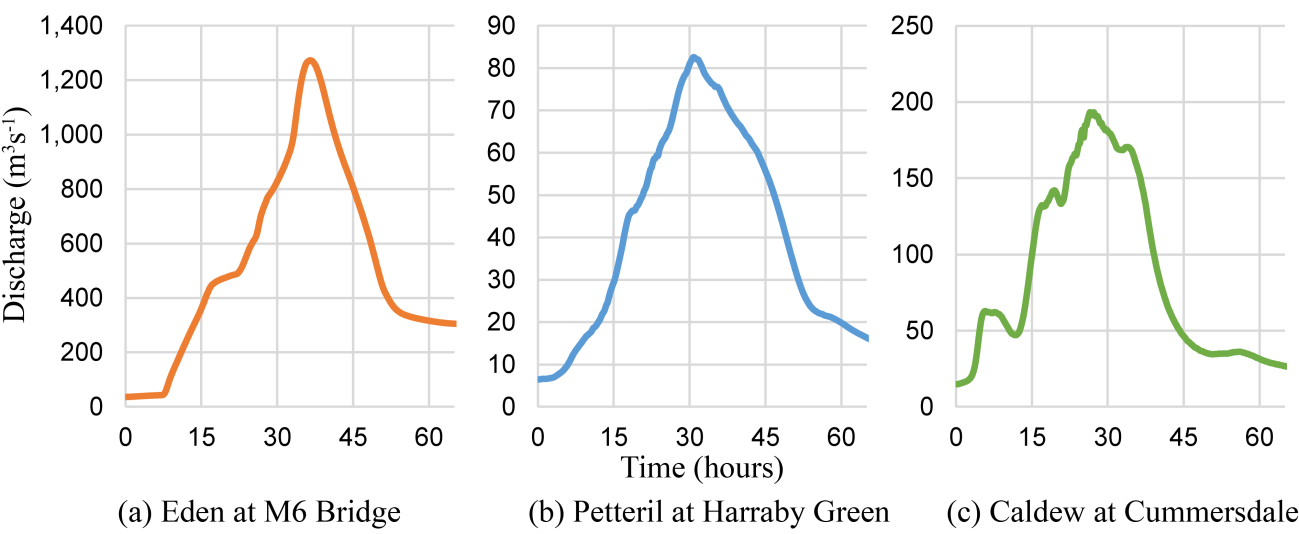
\includegraphics[width=0.9\textwidth]{Figure4.png}
\caption{Volumetric discharge inflow for the three rivers during the event.}
\label{BoundaryDischarges}
\end{figure*}

The topographic features, three rivers concerned, location of validation points, and approximate extent of the flood are shown in Figure \ref{CarlisleMap}. The root mean square error (RMSE) of the DGPS measurements is believed to be approximately 0.5m. The extent is deduced from a combination of EA records and the survey points, hence has buildings removed to create an appropriate mask for use with a high-resolution digital elevation model (DEM); for clarity this is different to the extent used by \citet{Horritt2010}. Inflow hydrographs for the three rivers are shown in Figure \ref{BoundaryDischarges}. The effects of rainfall within the city are neglected herein, to allow comparison with other published studies reproducing the event, and also because data is lacking for the sewer network and there is only anecdotal evidence detailing the sewer surcharging. 

The value of \(C\) in equation \eqref{CFL} is taken to be 0.5 for all simulations hereafter, to be consistent for all simulations, and accepting that some diffusion may occur, but the errors present in the input datasets are likely far more significant. The authors wish to emphasise that model stability should be ensured for values up to 1.0, and the value selected is purely based on prior experience and analytical test cases with shocks and discontinuities \citep{Liang2009c}. Simulations were run at 5 different spatial resolutions: 2m, 5m, 10m, 15m and 25m. A downstream depth condition is imposed on the River Eden at the western edge of the domain, extrapolated from the nearby Sheepmount gauging station and thus negating its value as a further validation control. The performance of each simulation is evaluated with respect to the RMSE for the DGPS survey points, which are compared against the simulated water level for the nearest inundated cell by straight-line distance. A fit statistic \(F\) is assessed against the extent, 

\begin{equation}
	\label{FitStatistic}
	F (\%) = \frac{A - B}{A + B + C} \times 100,
\end{equation}

where \(A\) is the number of correctly predicted as inundated cells, \(B\) the erroneously predicted as inundated cells, and \(C\) the erroneously predicted as dry cells \citep[as in][]{Horritt2010}. It should be noted that this metric, although well-established, exhibits a slight preference among erroneous cells for under- rather than over-estimation, which could penalise coarse resolution simulations where terrain averaging has removed obstructions from the floodplain.
Floodplain and channel Manning's \(n\) were independently varied between the ranges of 0.02 -- 0.06 and 0.02-- 0.08 respectively at 0.01 intervals, requiring 35 simulations per resolution and 175 in total. Observations during and after the flood suggest that levels on the River Caldew upstream of a disused railway bridge were increased at least in part by debris trapped under a bridge, and that the gas works area initially flooded as a result of wall collapse \citep{EnvironmentAgency2006a,Fewtrell2011a}, which is not considered within the model. Accordingly the bias is not considered a good measure of model performance; RMSE and F are the two metrics considered to be most appropriate. A non-stationary response to calibration is found for different resolutions. Calibration of Manning's \(n\) is based on selecting the parameter pair giving the lowest RMSE against the DGPS points. Selected river channel Manning's \(n\) were 0.060, 0.045, 0.020, 0.020, and 0.075 for resolutions 2m, 5m, 10m, 15m and 25m respectively. Floodplain values were 0.040, 0.050, 0.050, 0.020, and 0.020 in the same order. Maximum depths for the calibrated simulations are shown in Figure \ref{MaxDepths}, where it can clearly be seen that similar extents are attainable for all of the spatial resolutions considered herein. 

\begin{figure*}[tpb]
\centering
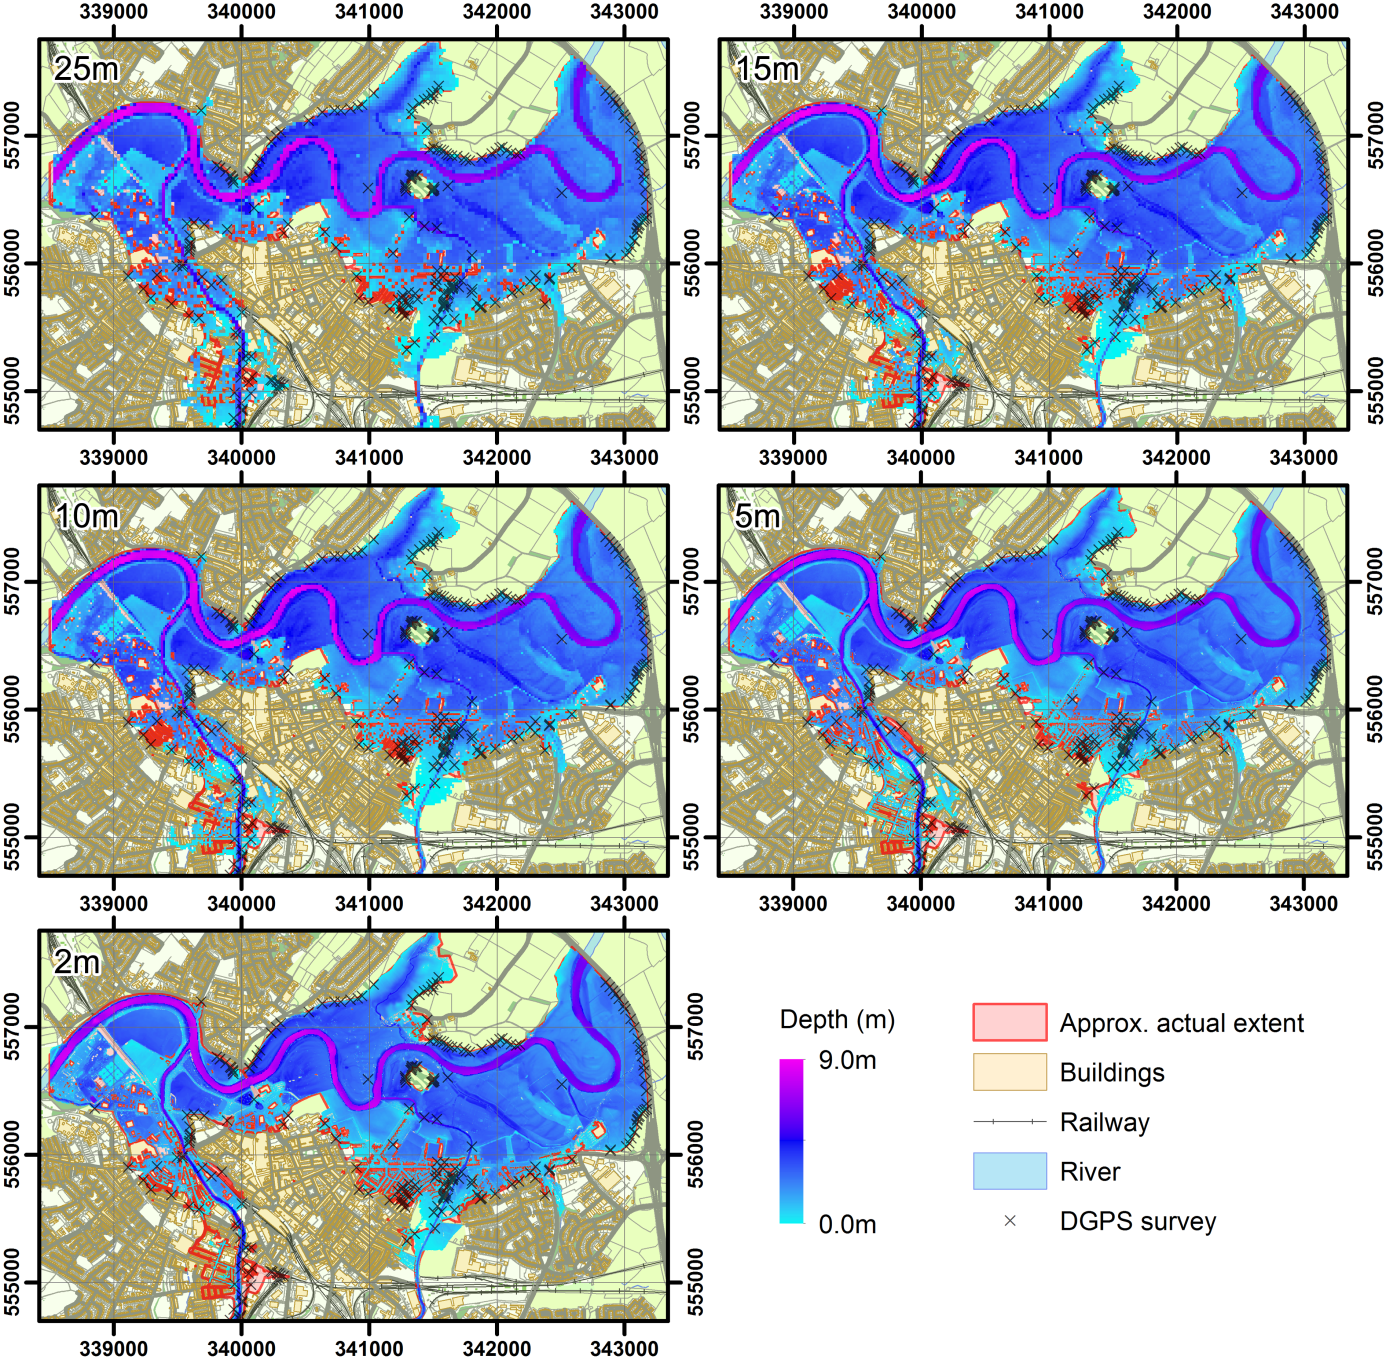
\includegraphics[width=1.0\textwidth]{Figure5.png}
\caption{Maximum depths for calibrated simulations at different spatial resolutions.}
\label{MaxDepths}
\end{figure*}
%\afterpage{\clearpage}
\begin{figure*}[tpb]
\centering
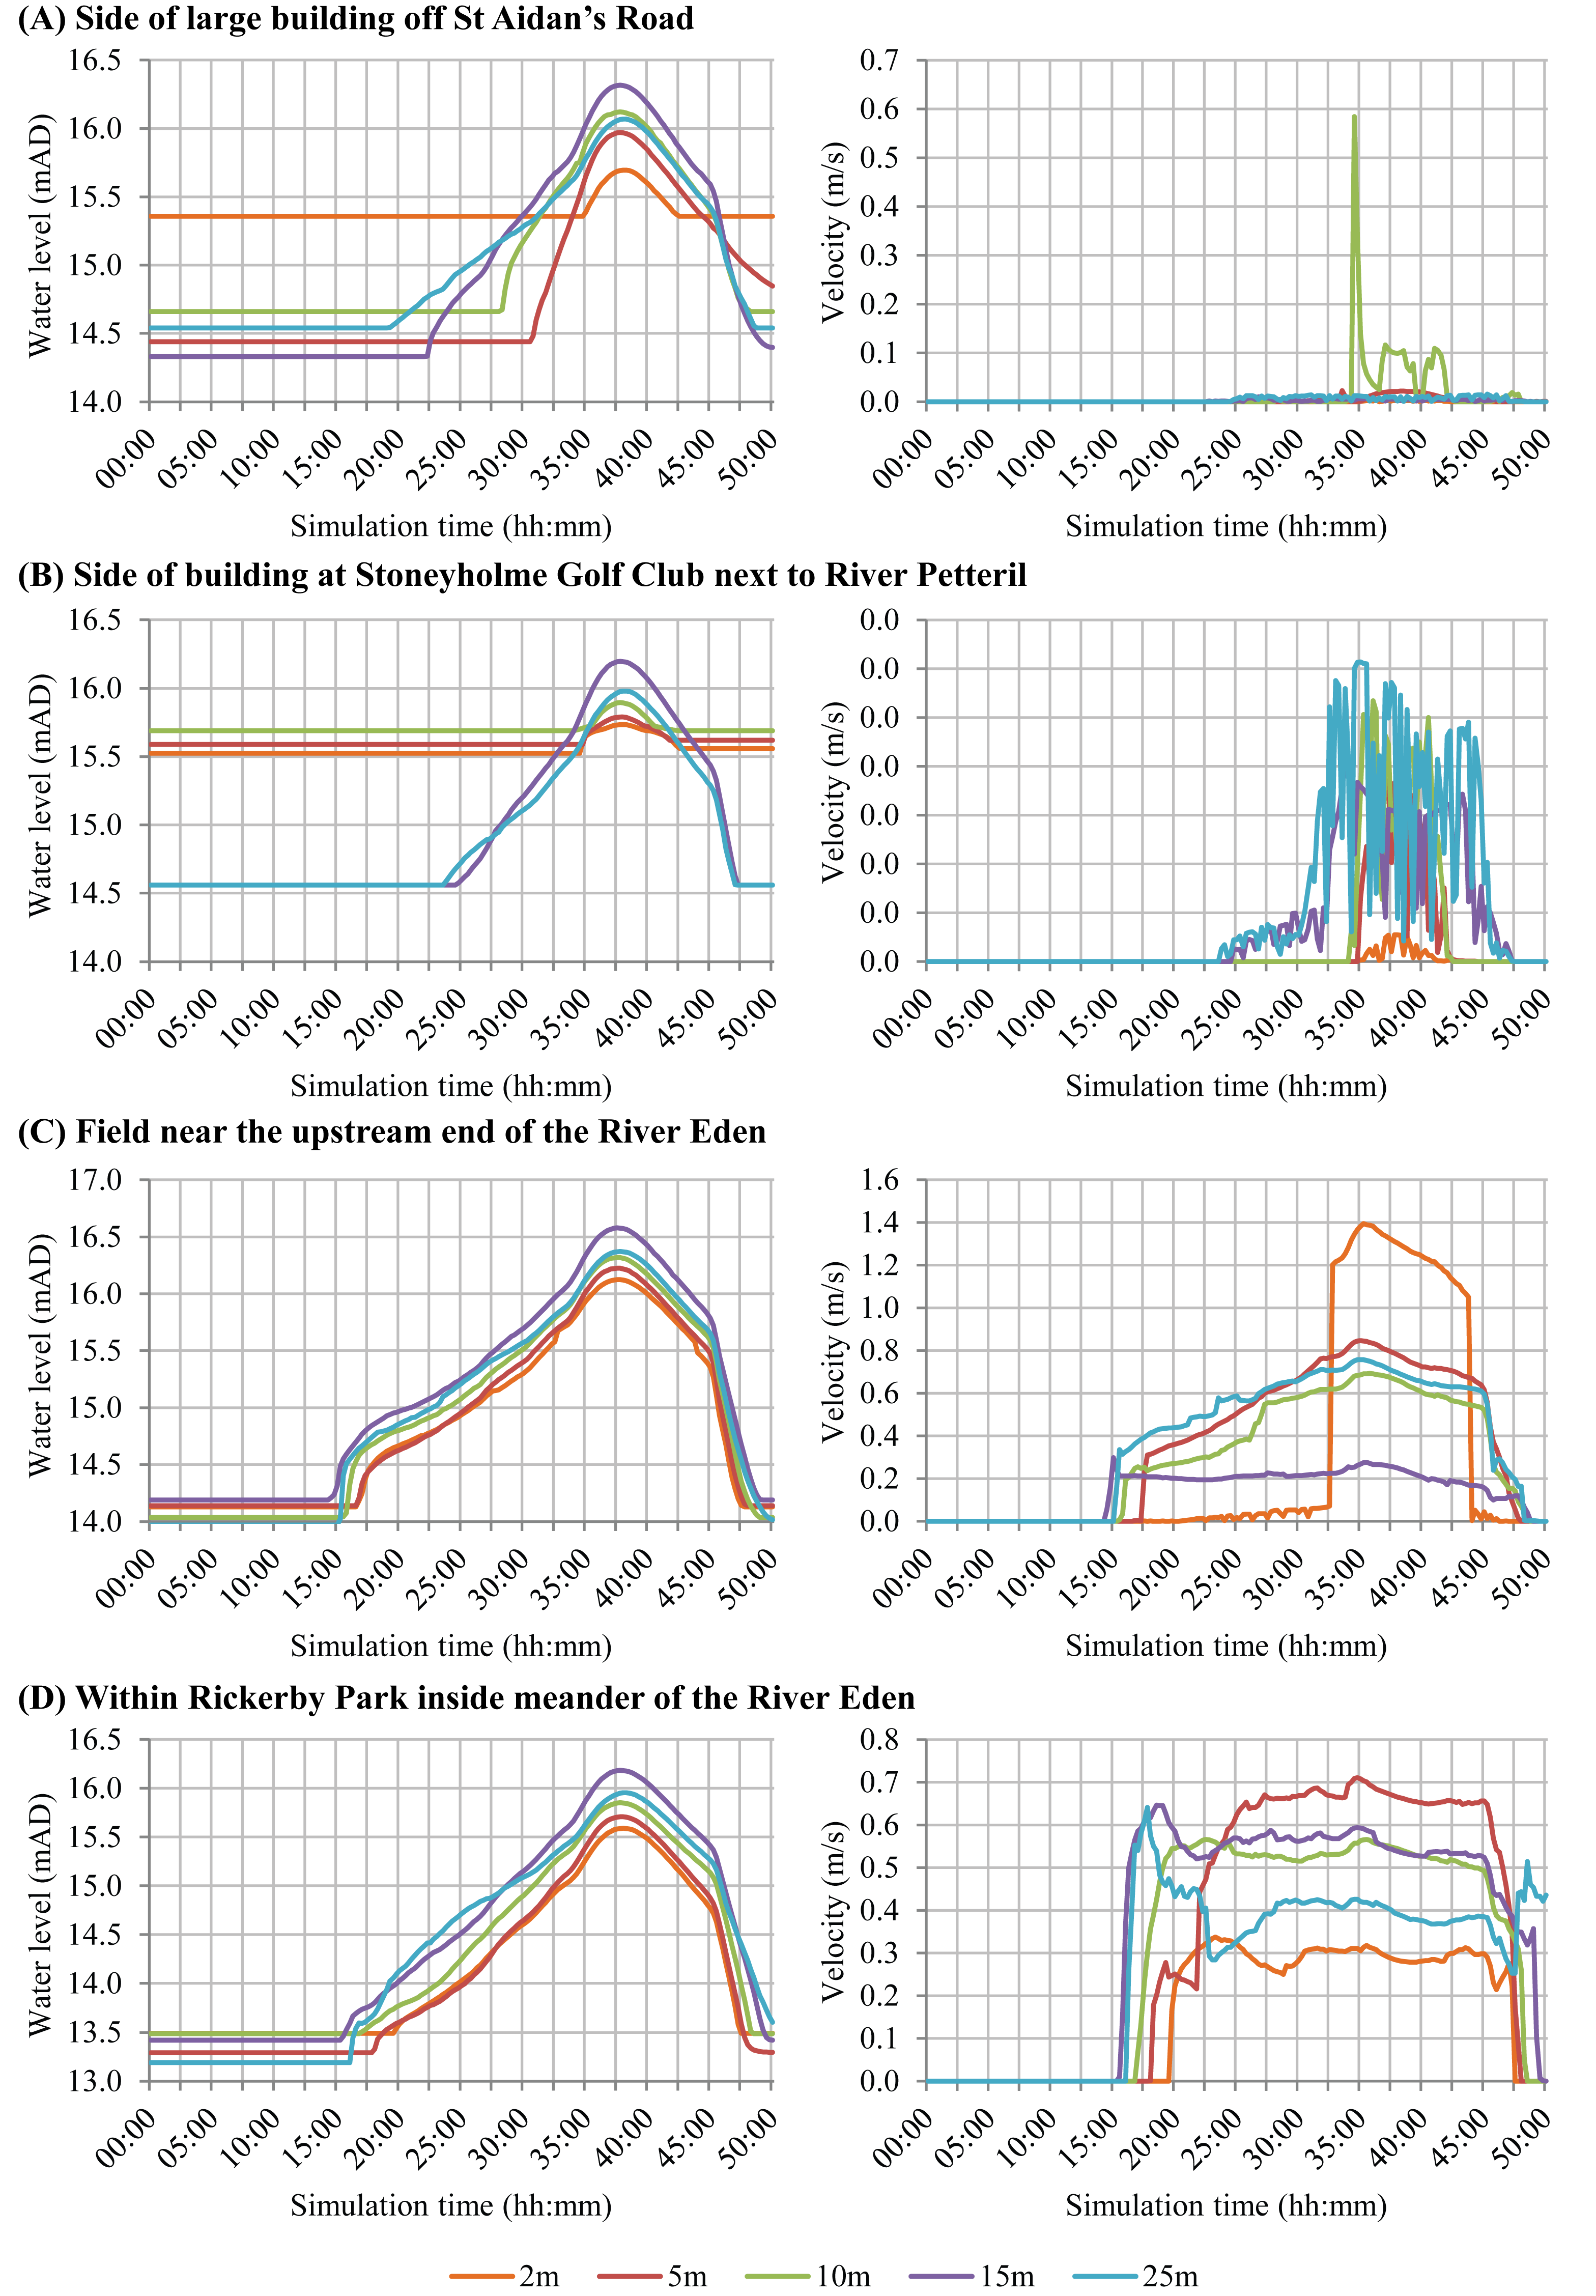
\includegraphics[width=0.93\textwidth]{Figure6.png}
\caption{Water level and velocity plots with respect to simulation time for the four sample points identified in Figure \ref{CarlisleMap}, with fixed Manning's \(n\) of 0.04.}
\label{TimeseriesPlots}
\end{figure*}
%\afterpage{\clearpage}

Timeseries plots of water levels and velocities at each resolution for the sample points shown in Figure \ref{CarlisleMap} are given in Figure \ref{TimeseriesPlots}, for a uniform Manning coefficient of 0.04 for the domain including the channel. Where the water level is flat at the start of a simulation, this indicates the bed elevation of the cell which is hence dry. Velocity results vary significantly between different resolutions, however no data exist to validate velocities. Low velocities would typically be expected at point A, which is far from the watercourses and within a residential area with obstructions. Close to the River Petteril at point B, there is clear evidence that velocities vary greatly at coarse resolutions, not unexpected given that the river is less than 5m wide at this point; crucially however the time of inundation at this point is incorrectly predicted at 15m and 25m resolutions.  At point C the levels are in broad agreement across all resolutions, however a clear jump in velocities is observed at 2m resolution, which is a result of flow eventually overtopping a wall in this location only represented in high-resolution data. Levels are also in agreement at point D, however velocities vary across a range with no clear trend against grid resolutions. The 2m grid resolution consistently produces the lowest floodplain velocities, except in the case of point C as described.

\begin{table*}[tpb]
\small
\centering
\caption{Simulation run-times for different devices, spatial resolutions and numerical precision (hh:mm:ss)}
\label{PerformanceResults}
\makebox[\linewidth]{
\begin{tabular}{llllllll}
\hline
			 		& 			& \multicolumn{2}{c}{NVIDIA Tesla M2075}			& \multicolumn{2}{c}{AMD FirePro V7800}			& \multicolumn{2}{c}{Intel Xeon E5-2609} 	\\
Resolution		 		& Cells		& 32-bit 		& 64-bit 		& 32-bit 		& 64-bit 		& 32-bit 		& 64-bit 	\\
\hline
25m					& 23,370		& 00:00:30	& 00:01:21	& 00:01:02	& 00:01:56	& 00:03:39	& 00:06:57 \\
15m					& 63,668		& 00:01:21	& 00:04:16	& 00:02:29	& 00:07:16	& 00:11:51	& 00:24:44 \\
10m					& 145,656		& 00:03:21	& 00:11:18	& 00:04:05	& 00:16:41	& 00:32:33	& 01:18:31 \\
5m					& 581,061		& 00:18:45	& 01:10:05	& 00:20:18	& 02:12:07	& 03:47:01	& 09:29:52 \\
2m					& 3,637,491	& 03:24:22	& 13:41:44	& 10:37:04	& \textit{\textgreater 40 hours}	& \textit{Not tested}	& \textit{Not tested} \\
\hline
\end{tabular}
}
\end{table*}

The calibrated simulations were executed with three different processing devices from each of the mainstream vendors to compare run-times. The time taken to simulate the first 50 hours of the event, long enough to obtain the maximum extent, is given in Table \ref{PerformanceResults}. CPU simulations at high resolutions even using all four cores of the Intel Xeon E5-2609 would have taken several days to complete, hence were not run to completion. By contrast, an NVIDIA Tesla M2075 intended for scientific computing reduces the run-time to less than 3.5 hours or 14 hours for 32- and 64-bit floating-point computation respectively. The vendor-quoted computational power of the two devices is 77 gigaflops (floating point operations per second) for the Intel Xeon E5-2609 \citep{IntelCorporation2012}, and 515 for the NVIDIA Tesla M2075 \citep{NVIDIACorporation2011}, representing a theoretical improvement of 6.7 times for the scientific GPU. Free-surface levels and velocities are sufficiently small for this case to allow good numerical resolution and only minor differences in inundation extent when comparing 32-bit to 64-bit results. The authors wish to emphasise that this is not true for the general case and sensitivity analysis is always necessary before discarding 64-bit precision. We suggest that the narrowing performance gap between NVIDIA and AMD devices with increasing resolution is a consequence of the overhead associated with launching a kernel, which becomes an increasingly small percentage of the total time. There are many factors influencing performance however. The AMD GPU is installed in a conventional workstation, and exhibits substantially reduced performance in simulations lasting more than an hour (i.e. 2m and 5m 64-bit), believed to result from hardware performance throttling because of high temperatures.

All simulations in Table \ref{PerformanceResults} were carried with using OpenCL, using all processing power and cores available for each device. Consequently even the processing time with the Intel Xeon E5-2609 CPU (quad-core with hyper-threading) represents a major reduction over many of the hydraulic modelling software packages currently used in industry, which offer no parallelisation or have been retrospectively parallelised in part using OpenMP \citep{Pender2010,Pender2013} where significant portions of code still execute serially and Amdahl's Law limits the performance increases. As expected for devices compliant with relevant IEEE standards for floating-point computation, there is no difference between the results obtained using the three different processing devices. 

As a purely indicative representation of the performance scaling achieved, the same numerical scheme programmed in FORTRAN95 and executed on a single core of the same CPU required 4.10 hours for the 10m 64-bit precision simulation. The software presented herein therefore reduces simulation times by approximately 3.1 times for the multi-core CPU and 21.8 times by using a high-end GPU for this simulation. The authors caution that this comparison with FORTRAN95 code should not be construed as precise; software performance on any processing device is a function of the programmer's skill, compiler used, degree of optimisation, memory access patterns, and numerous other factors. The magnitude of the speed-up with OpenCL for GPU devices is also seen to scale with increasing domain size, from 5.1 times at 25m to 8.1 times at 5m resolution, when comparing the Intel Xeon to the NVIDIA Tesla. Speed-up is dependent on a number of factors, but amongst the most significant is the proportion of dry cells; the overhead associated with launching a kernel and transferring data to registers for evaluation remains constant, but for dry cells kernels are permitted to exit early and this overhead is proportionally larger. Greater levels of speed-up relative to CPUs could be achieved for a larger domain with more immediate inundation (i.e. flash flooding), but likewise GPU computation may in fact be slower for very small domains at coarse resolutions.

\begin{figure*}[tpb]
\centering
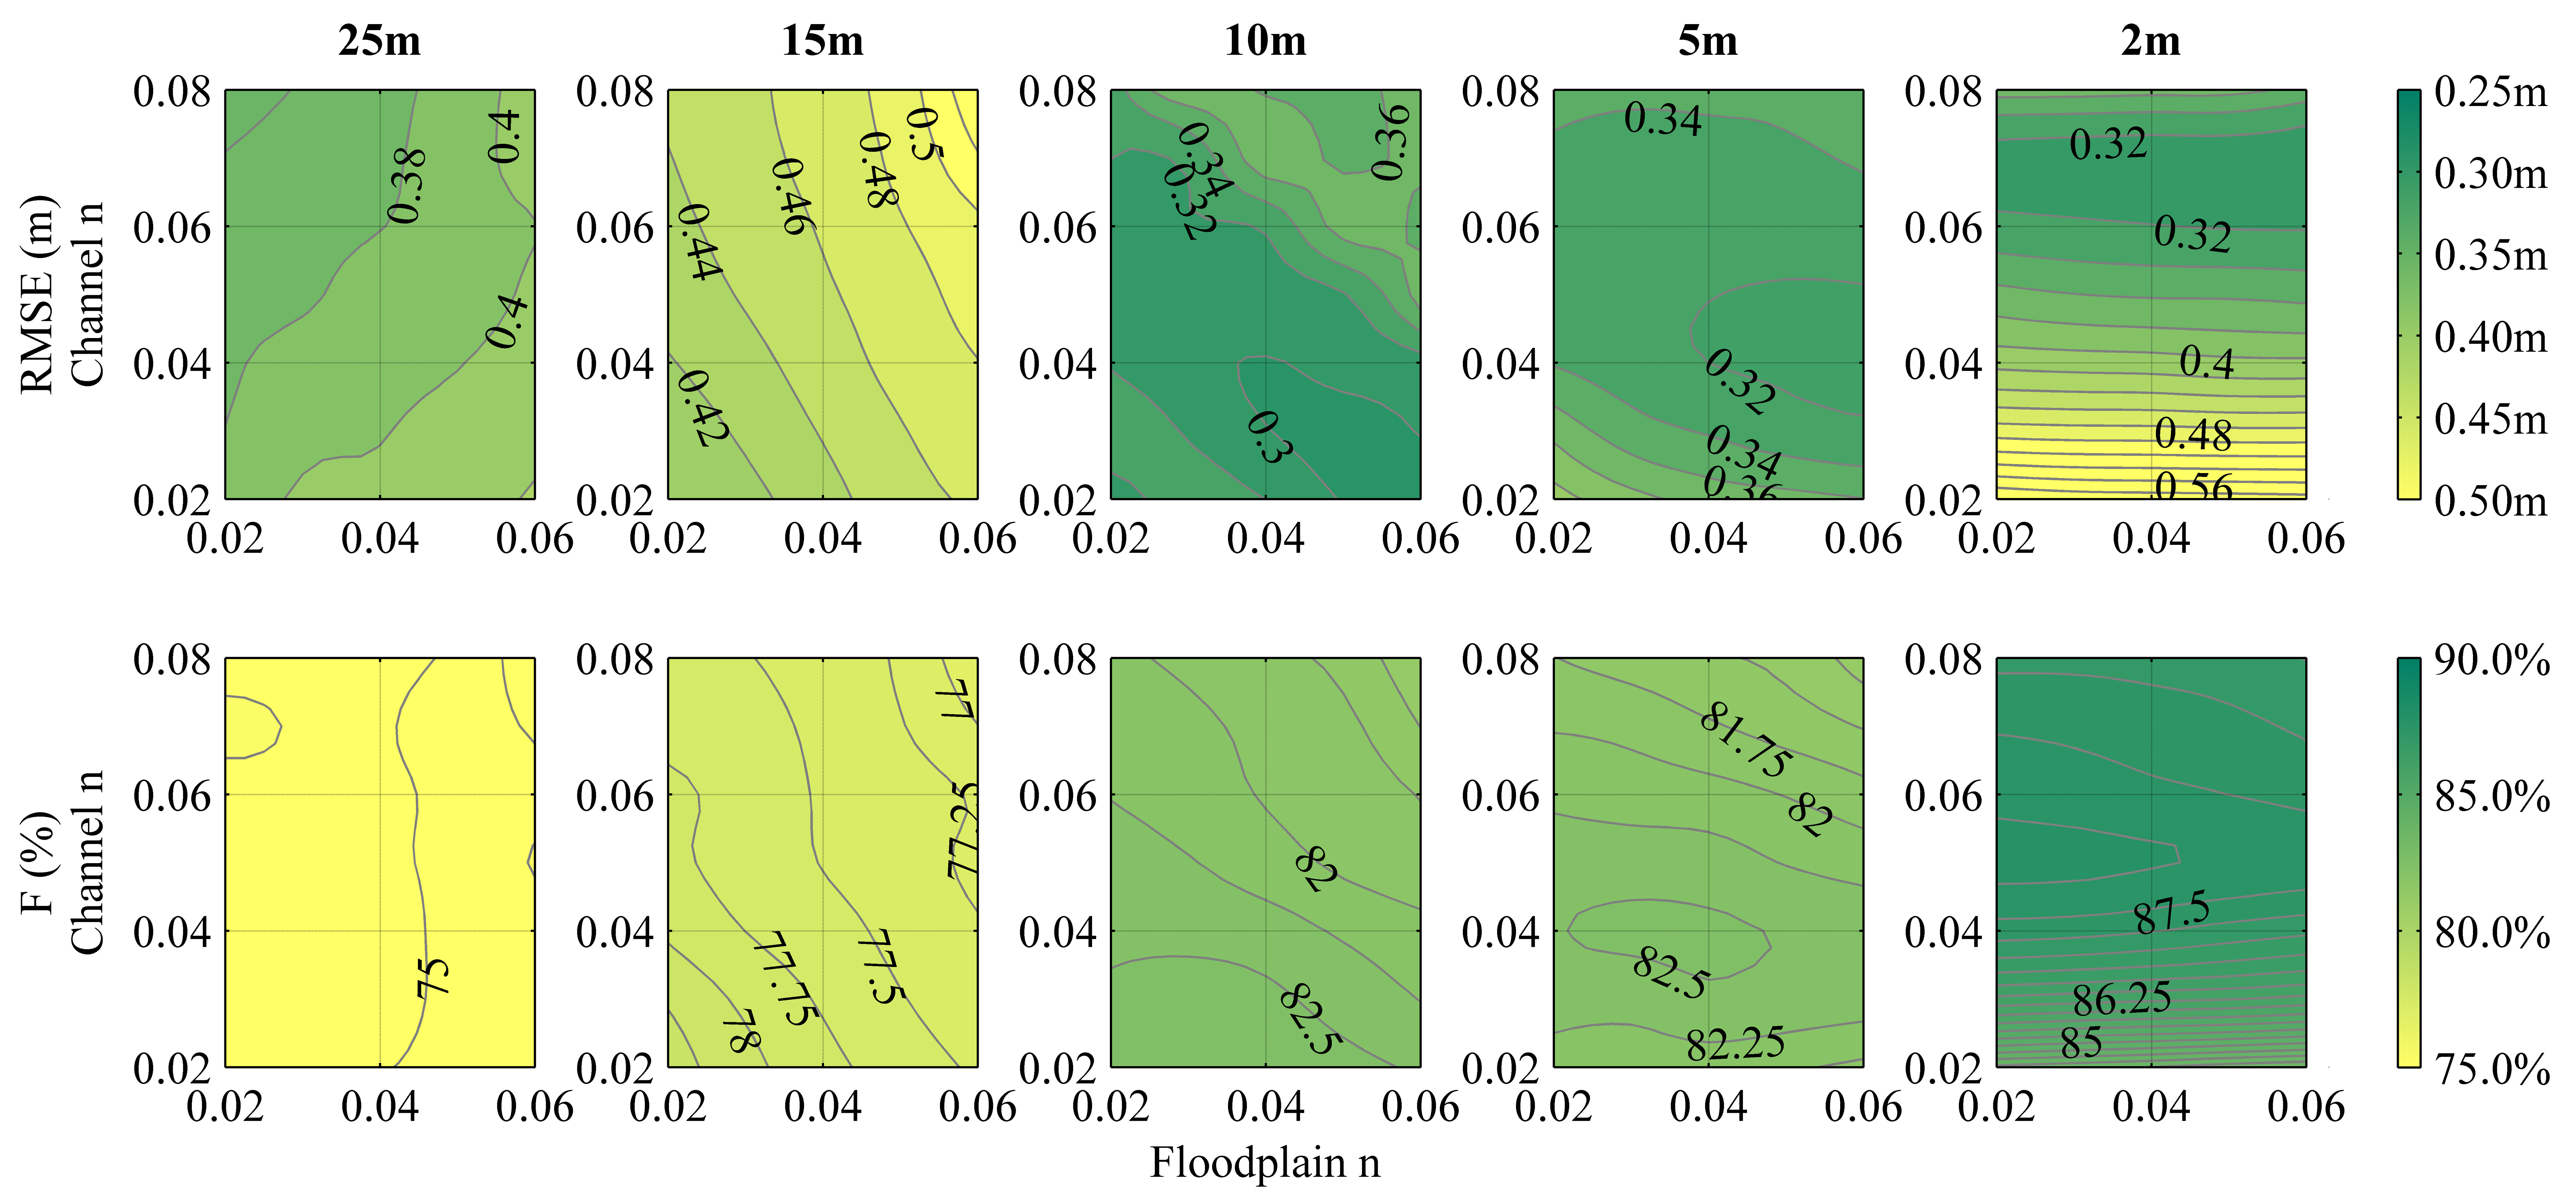
\includegraphics[width=1.0\textwidth]{Figure7.png}
\caption{Parametric calibration for variations of Manning’s n within the channel and floodplain.}
\label{Calibration}
\end{figure*}
\begin{figure*}[tpb]
\centering
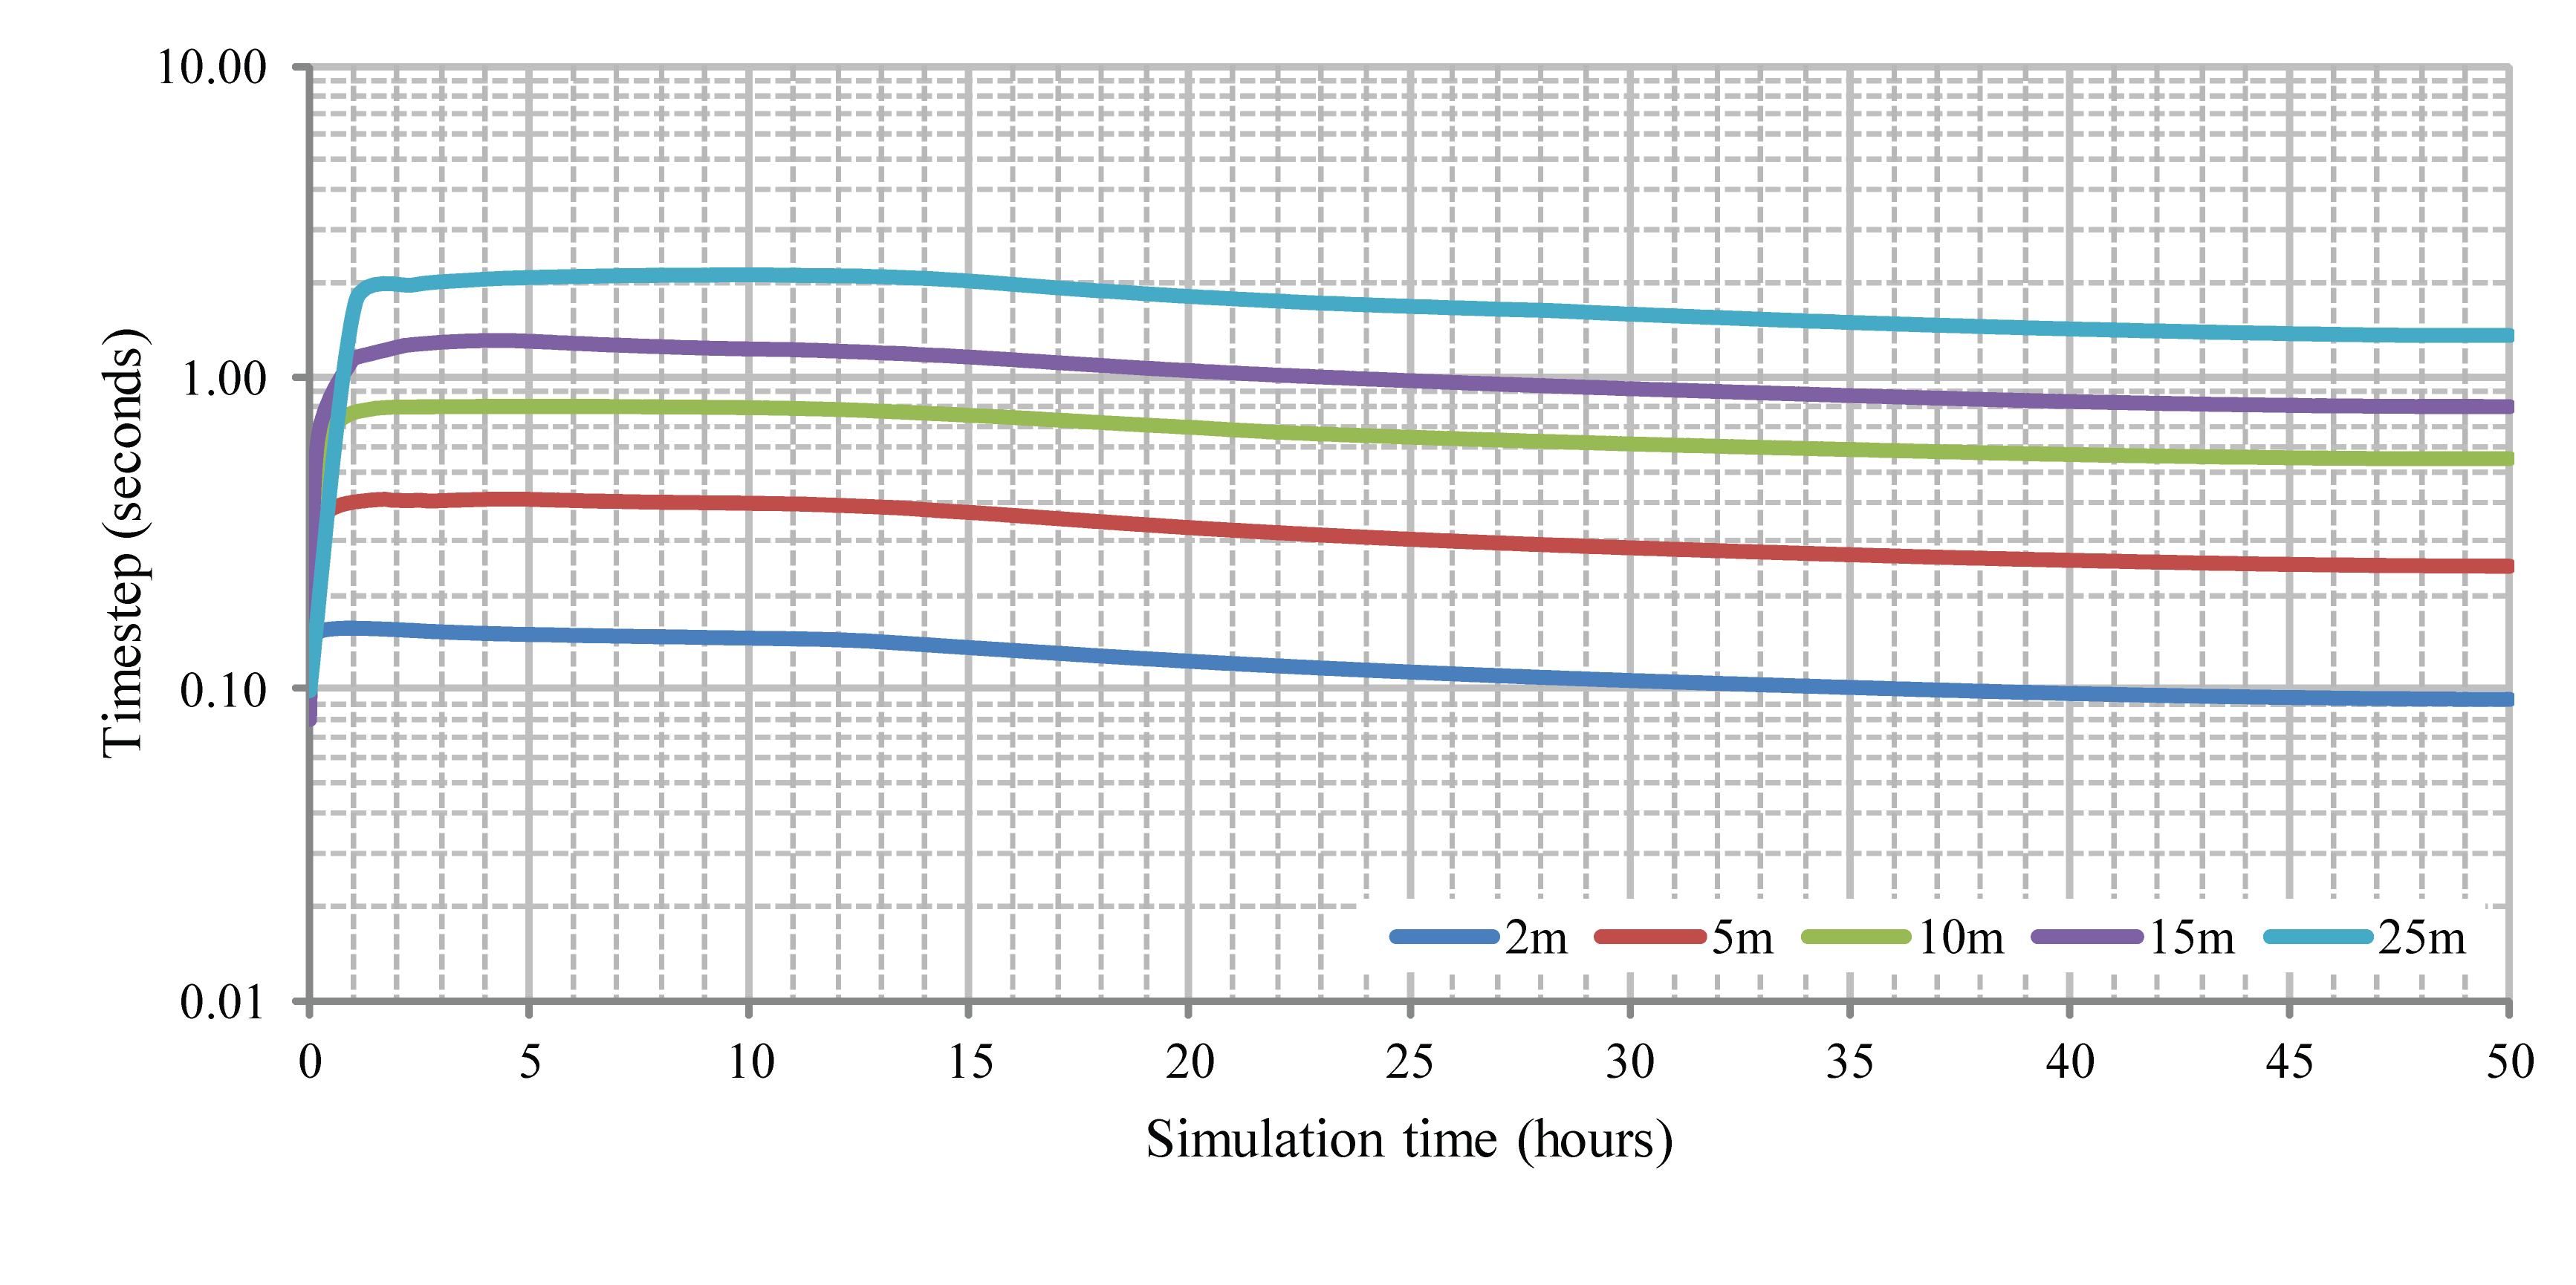
\includegraphics[width=1.0\textwidth]{Figure8.png}
\caption{Model timesteps used throughout 64-bit simulations at different resolutions.}
\label{Timesteps}
\end{figure*}

Further exploration of sensitivity to Manning coefficients yields interesting results. Contour plots for the biparametric calibration with the key performance metrics are shown in Figure \ref{Calibration}. Almost all of the simulations give an RMSE less than the estimated error in the DGPS measurements. At coarse resolutions optimum performance with respect to RMSE and F are not coincident. There is no consistent trend in the pattern of the optimal zones, as the resulting topography after interpolation can vary greatly at coarse resolutions owing to the size and positioning of buildings. For an increasingly fine grid, clear optimal zones emerge at 10m and 5m resolution, and by 2m only an optimal channel coefficient can justifiably be identified. For clarity at coarse resolutions no optimal zones could be found outside the calibration limits. Moreover the sensitivity changes in nature; higher resolutions show a decreasing sensitivity to the floodplain Manning's \(n\) and increased sensitivity for the channel. At 2m resolution sensitivity for the floodplain is so low that floodplain calibration barely influences the results and channel flows become the dominant factor, as confirmed by the lower velocities on the floodplain shown in Figure \ref{TimeseriesPlots} except at point C where a wall is eventually over-topped. This is not unexpected, velocities should be low for a fluvial inundation of this type, and given the meandering channel a high spatial resolution allows variations in flow characteristics within cross-sections to be properly considered. Closer examination of velocities at different intervals in the simulation shows that at coarse resolutions the flow is often circumventing the main channel due to the Cartesian grid and winding channel. Flow therefore enters the floodplain (especially in the meanders in the centre of Figure \ref{CarlisleMap} around point D) at a higher velocity, and the sensitivity to Manning's \(n\) is accordingly higher in these areas. If the low floodplain sensitivity holds more generally in the context of other flood events, there is clear potential for high-resolution hydrodynamic modelling with the full shallow water equations to improve accuracy for SuDS design, especially with hypothetical events. The combination of high grid resolutions and velocities in the main channel affect the timesteps shown in Figure \ref{Timesteps}, which can be as small as 0.093 seconds for the 2m simulation. 

\section{Conclusions}

The software presented herein is successfully applied to reproduce the flooding which occurred in Carlisle during 2005. The same approach can easily be used to model surface water flooding, and to assess the impact of potential SuDS designs. Further improvement in the accuracy of the simulations would be difficult to assess given the error inherently present in the validation datasets. GPUs have allowed high-resolution simulations to be carried out with a robust and physically accurate numerical approach for hydrodynamic modelling in a matter of hours rather than days. The techniques adopted capitalise on parallel processing with the flexibility to operate across a wide range of devices currently available from mainstream hardware vendors; software developers for hydrodynamic models must respond to the stagnation of processor clock speeds and harness parallelism to take advantage of the most recent increases in computing power. 

High-resolution modelling has accurately represented and constrained the complex flow dynamics to within the river channel, and as a consequence we have observed decreasing sensitivity for the floodplain with higher resolutions, resulting in extremely low sensitivity at 2m resolution. This demonstrates the importance of accurately representing the topography within hydrodynamic models, but overland flow velocities might be higher during surface water flooding. Further work is required to corroborate and explore parametric sensitivity. Different types of urban flood events should be simulated with high spatial resolutions and parametric sensitivity examined. The authors also intend to extend the software to use multiple GPUs for a single simulation, and will provide details in a forthcoming publication.

\section*{Acknowledgements}
Gratitude is expressed to Dr Jeff Neal of Bristol University and his colleagues, and the Environment Agency for collecting and supplying necessary data.

\section*{Funding}
The authors are grateful to Advanced Micro Devices Inc. for supplying the AMD FirePro V7800 GPU device. The NVIDIA Tesla M2075 device used is part of a larger system funded by the UK Engineering and Physical Sciences Research Council (EP/K031678/1).

\bibliographystyle{apalike}
\bibliography{Paper}

\end{document}